\documentclass{article}
\usepackage{graphicx}
\graphicspath{ {images/} }
\title{Deep Q Learning for Rocket Landing}
\date{March 2018}
\author{Ibis Prevedello}

\begin{document}
\maketitle

\section{Introduction}
The goal of this project is to study and implement a Reinforcement Learning algorithm in order to solve several games from the Gym toolkit. The algorithm chosen is Deep Q Learning, which uses a Deep Neural Network to learn the Q Function, also some improvements are tried with Double Deep Q Learning and Prioritized Replay.

\section{Description of the problem}
Besides the idea to develop an algorithm that could be used for more than one game, this report will contain only the solution for the environment called 'Rocket Landing', which is inspired on SpaceX idea of reusable rockets.

\begin{figure}[h]
\centering
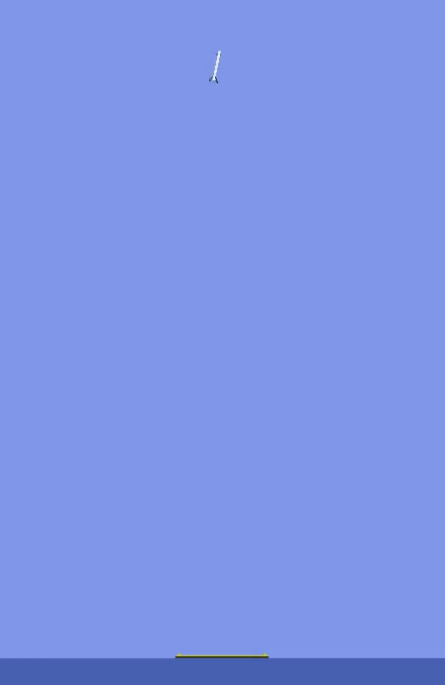
\includegraphics[scale=0.30]{environment}
\caption{Game screenshot}
\label{fig:fig1}
\end{figure}

The rocket starts from a high altitude, out of the screen, as show in image \ref{fig:fig1}, and the goal is to control it using the trusters in order to land it on a drone on the sea. The landing also needs to occur smootly in order to avoid demaging the rocket legs.

\section{Formal model of the problem}
In order to control the rocket it is necessary to give to the learning algorithm some data, called state variables and take one of the actions from the control inputs.
After every iteration, which is a frame of the simulation, an action will be calculated and a result of that action will be returned to the algorithm.

\subsection{State variables}
For the State variables, it is possible to limit the number of variables used for the training, however it was decided to use all the data available in order to have a better control of the rocket.

\begin{itemize}
	\item x position
    \item y position
    \item angle
    \item first leg ground contact indicator
    \item second leg ground contact indicator
    \item throttle
    \item engine gimbal
	\item x velocity
    \item y velocity
    \item angular velocity
\end{itemize}

\subsection{Control inputs}
Using this simulator it is possible to chose one of the two types of controls, or discrete or continuous. It was decided to use discrete control because the same code could be used to a bigger variety of other simulators inside Gym.

\begin{itemize}
	\item gimbal left
    \item gimbal right
    \item throttle up
    \item throttle down
    \item use first control thruster
    \item use second control thruster
    \item no action
\end{itemize}

\section{Solution algorithm}
A algorithm well known is the Q Learning, where a table is created with the size of its action and states, and the values of the table are updated based on the learning process.

\subsection{Hyperparameters}
The hyperparameters used for this project are presented in the table below:

\begin{center}
\begin{tabular}{ |c|c| } 
 \hline
 \textbf{Parameter} & \textbf{Value} \\ 
 \hline
 $\gamma$ (reward discout factor) & 0.99 \\ 
 learning rate & 0.00025 \\
 target update (episodes) & 1000 \\ 
 $\epsilon$ start & 1.0 \\ 
 $\epsilon$ end & 0.01 \\ 
 $\epsilon$ decay & 0.0001 \\ 
 batch size & 128 \\ 
 memory capacity & 200000 \\ 
 \hline
\end{tabular}
\end{center}



\subsection{Experience replay}

\section{Implementation}
The algorithm here described is divided in tree different parts, the memory, the brain and the agent. Each one has its own well defined role and it is important to keep the code separated and organized.

\subsection{Memory}
The memory is necessary to keep in memory a certain number of last actions executed by the agent. It is necessary to store the experience that will be used for Experience Replay.

The Experience Replay is a stratagy used to train the Neural Network not only based on the last experience, but on a batch with multiple experiences saved in the memory. For this part there are multiple ways to select this samples from the memory, random samples are one, and other more efficient algorithm is to determine an error for each sample and select those with a hier error.

Each experience saved to the memory have the following information:

\begin{itemize}
	\item current state
	\item action
	\item reward
	\item next state
\end{itemize}

\subsection{Brain}
The Brain class encapsulates the Neural Network. It was defined with 2 hidden layers with 256 neurons each and ReLU activation function. The input number of neurons is the number of states and the output number of neuros is the number of actions.

This network is trained in order to aproximate the Q function and the target model is a simple copy of the model, however it is updated sporadically, after 1000 steps.

For the loss it is using the Huber loss function, it is a loss function used in robust regression, that is less sensitive to outliers in data than the squared error loss.

\subsection{Agent}
The Agent class is a container that encapsulates all the methods for the algorithm to run, such as the act, observe, replay and epsilon decrement.

Also some more higher level tasks are also implemented like save and load model, which enables the script to stop training and continue it from where it stopped.

\section{Results}
The first data that is useful to analize is the evolution of rewards over the training. In image \ref{fig:fig2} is plotted this evolution and it is possible to see the the reward is improving over time, even though

\begin{figure}[h]
\centering
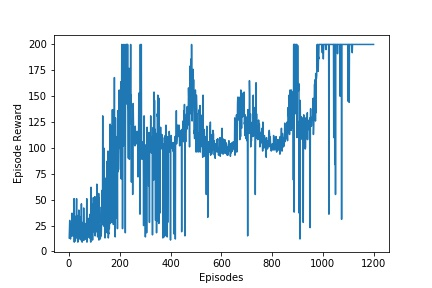
\includegraphics[scale=0.5]{rewardOverEpisodes}
\caption{Reward over episodes}
\label{fig:fig2}
\end{figure}

\section{Conclusions}
Another option 

\end{document}
